\documentclass[11pt]{report}
\usepackage[margin=1in]{geometry}
\usepackage{titlesec}
\usepackage{graphicx}
\usepackage{parskip}
\usepackage{glossaries}

\titleformat{\chapter}{\Large\bfseries}{}{0pt}{\huge}
\titlespacing\chapter{0pt}{*1}{*1}
\titlespacing\section{0pt}{*0}{*0}
\titlespacing\subsection{0pt}{*0}{*0}
\titlespacing\paragraph{0pt}{*0}{*3}

\newcommand*{\TitleFont}{
      \usefont{\encodingdefault}{\rmdefault}{b}{n}
      \fontsize{24}{36}
      \selectfont
}

\newacronym{2d}{2-D}{Two-Dimensional}
\newacronym{3d}{3-D}{Three-Dimensional}
\newacronym{cnc}{CNC}{Computer Numerical Control}
\newacronym{pcb}{PCB}{Printed Circuit Board}

\title{\TitleFont Delta Robot \\ Project Definition}
\author{
	Evan Milton \\
	Computer and Electronics Engineering \\
	University of Nebraska at Lincoln - Omaha Campus \\
	Electronics Engineering
		\and
	Josh DeWitt \\
	Computer and Electronics Engineering \\
	University of Nebraska at Lincoln - Omaha Campus \\
	Computer Engineering and Mathematics, minor in Computer Science
		\and
	Chad Staley \\
	Computer and Electronics Engineering \\
	University of Nebraska at Lincoln - Omaha Campus \\
	Electronics Engineering
		\and
	James Gehringer \\
	Computer and Electronics Engineering \\
	University of Nebraska at Lincoln - Omaha Campus \\
	Computer Engineering, minor in Computer Science
}
\date{\today}

\begin{document}
\maketitle

\tableofcontents

\listoffigures
\begingroup
\let\clearpage\relax
\listoftables
\endgroup

\chapter{Background Summary}
\section{Statement of Need}
For many years, the human-machine interface has maintained a standard formula.
Persons are limited to point and click technology as their only means by which to interact with the digital realm.
As technology has advanced, new alternatives have emerged to allow  greater freedom of control, and although many of these devices are available to consumers, there has not been a push to combine them in ways that are intuitive and natural to use.

There is also a need for a faster and more configurable \gls{cnc}.
Most \gls{cnc}s found on the consumer market are slow~ causing the 'rapid prototyping' phase of development to suffer correspondingly.
A faster, more robust robot would cut down on project time and open the door for other applications.
Reconfiguration will help the technology to adapt and stay relevant.

One application possible with an improved interface and more robust robotics would be \gls{pcb} repair.
As components shrink in size, they become more difficult to manipulate.
When this is compounded with the complexities inherent in soldering, it can become dangerous to perform standard \gls{pcb} repairs.
Although industry has already solved the problem of component placement for bare circuit boards, no device yet exists that allows persons to utilize the precision of robotics in this area. 

\section{Research Summary}
The Delta Robot to be used as the foundation for this 2014 Capstone Project was inspired by several recent trends in robotics.
The OpenBeam Kossel Pro is a 2012 project that uses a delta robot for \gls{3d} printing, much like its open-source counterpart, the Rostock.
While both represent breakthroughs in Delta Robot application, its origination in industry as a rapid placement device on assembly lines suggests that the architecture is capable of much more complex tasks.

One of the Delta Robot's primary advantages over a standard \gls{cnc} is the increased degree of freedom that comes with independently controlled axes.
While several industrial robots take advantage of this fact, their price can fluctuate in excess of \$50,000.
There are currently no commercially available Delta Robots that are affordable, precise, customizable, and open source.

Fortunately, recent advances in the human-machine interface have countered stagnation in consumer robotics.
The Oculus Rift is one such revelation; a virtual reality helmet that can handle \gls{3d} output through stereoscopic vision.
The helmet also has motion sensors to be able to sense where a user would like to look or change focus to, enabling total immersion in a digital world.

The Leap Motion is another new technology that is reshaping how humans interact with machines.
The Leap Motion is a control interface that is touch free.
The Leap has a work area monitored by infrared sensors that can track many objects, but specifically had hands in mind.
The Leap can track multiple hands and each finger individually.
This technology has been used in many applications, from replacing a mouse to controlling a robotic hand.
Its versatility has the potential to be useful, especially as its availability and community grows.

When a human tries to perform a task, there is one limiting factor: the human's fine motor skills are limited by what they can see.
When a human looks into a microscope, it is very easy for them to manipulate small items with tweezers.
Increasing the resolution of what a human can see will increase the resolution of what a human can manipulate.
In combining the above technologies, this 2014 Senior Capstone Project seeks to overcome many of the challenges faces by those with limited vision and movement capabilities.

\section{System Requirements}
Marketing requirements have been determined after performing background research on the subject, taking into special consideration the limitations of existing \gls{cnc} machines in existence today. Engineering requirements were derived from background research and the marketing requirements. 

\subsection{Stakeholder Chart}
The Stakeholder Chart is shown in Figure ~\ref{fig:stakeholderchart}. Note that the hardware engineer and software engineer report to both the systems engineer and the resource manager. In the event of a conflict on instructions from the systems engineer and the resource manager, the conflict will be discussed by the systems engineer and the resource manager, though the resource manager makes the final decision. 
\begin{figure}[h]
	\centering
	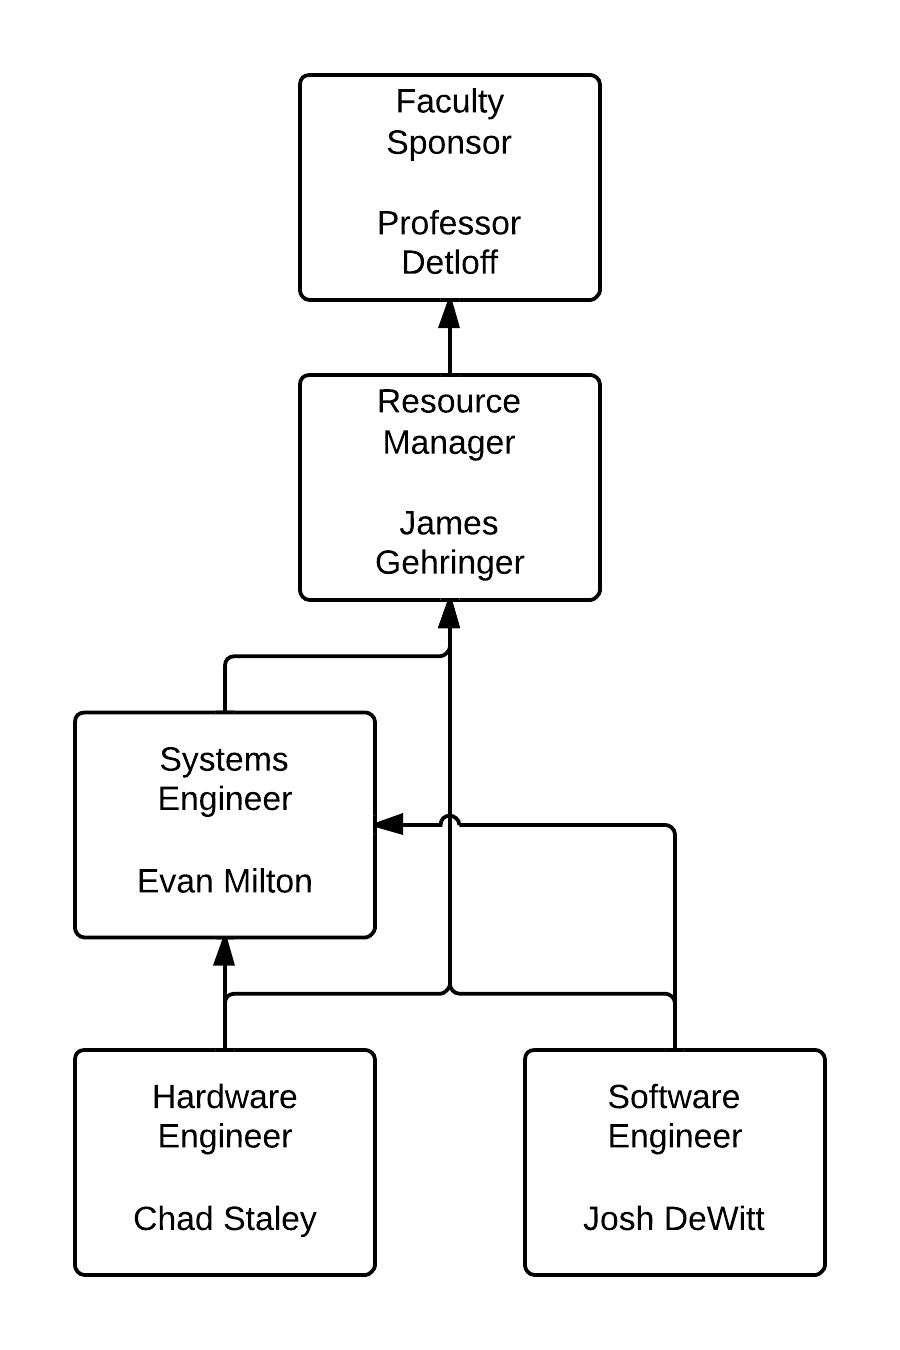
\includegraphics[width=0.5\textwidth]{organization.png}
	\caption{Stakeholder Chart}
	\label{fig:stakeholderchart}
\end{figure}

\subsection{Marketing Requirements}
The system will meet the following criteria:
\begin{enumerate} \parskip2pt
	\item be intuitive.
	\item act predictably.
	\item have an ergonomic design.
	\item have a simple interface.
	\item automatically configuration itself.
	\item be robust.
	\item have a modular design.
	\item operate safely.
	\item not harm humans.
	\item not harm itself.
	\item be able to recover from unexpected occurrences.
	\item be versatile in its uses.
	\item be able to be used for multiple applications.
	\item be able to use multiple interfaces for communication.
	\item be open source.
\end{enumerate}

\subsection{Engineering Requirements}
The system will meet the following criteria:
\begin{enumerate} \parskip2pt
	\item Performance
	\begin{enumerate}
		\item have an accuracy finer than 0.025 mm.
		\item have a resolution finer than 0.25 mm.
		\item have a work area 50 cm in diameter and 50 cm in height.
		\item travel faster than 500 mm per minute.
	\end{enumerate}

	\item Environmental
	\begin{enumerate}
		\item be transportable by two or fewer persons.
		\item produce less than 85 dB of sound from a distance of 3 feet.
	\end{enumerate}

	\item Health and Safety
	\begin{enumerate}
		\item have thermal shutdown and over-current protection.
		\item have a readily accessible emergency stop switch.
		\item halt all motion if a user enters the work area.
	\end{enumerate}

	\item Reliability
	\begin{enumerate}
		\item have critical components shielded from the work area.
		\item be modular in construction.
		\item use standard components.
		\item be vibration resistant.
		\item be able to run for 8 continuous hours of operation.
	\end{enumerate}

	\item Interfacing
	\begin{enumerate}
		\item be compatible with current G-code standards.
		\item have no more than five menus.
		\item have Ethernet compatibility.
	\end{enumerate}
\end{enumerate}

\subsection{Required Resources}
The persons involved with this project will require a dedicated collaborative space where regular meetings can be held, and items remain posted between sessions.
A lab environment equipped with computers containing necessary software, and soldering stations will be required for the hardware design and construction.
The software development can be done through any computer that has the proper tools installed, which depends upon the hardware chosen for the project.
Financial resources required will be determined upon initial analysis of the project requirements, but should not exceed \$2,500.

\chapter{Project Boundaries}
\section{Statement of Scope}
The Project will contain the following aspects.

\subsection{Human-Machine Interface}
It is the primary goal of this 2014 Capstone Project to improve the human machine interface through the addition of \gls{3d} visualization and \gls{3d} manipulation capabilities not currently implemented in industry and consumer electronics.
Students will seek to build upon recent commercially available technology, and combine it in new ways to create an interface that is intuitive, versatile, and robust.

\paragraph{\gls{3d} Visualization}
Modern mechanical interfaces generally employ \gls{2d} methods (computer monitors) in order to render a machine's world view.
2d visualization causes problems in orientation and perception, as the end-user is unable to discern crucial depth information from a single point source.
This project seeks to solve issues in orientation and depth perception through the use of a \gls{3d} display interface that presents to the user the data necessary to navigate in 3 dimensions.

\paragraph{\gls{3d} Manipulation}
Following the same logic, this 2014 Capstone Project also seeks to alleviate common control issues in machine interfaces based upon \gls{2d} button or joystick systems.
Allowing the end user to operate in real space will enhance control, stability, and ease of use for the final system.

\subsection{Application of Interface}
While the ability to control machinery in real space may ultimately yield many implementations, members involved with this project seek to demonstrate its abilities in the construction of a system by which minute electronic repairs may be examined and performed.
This system will utilize the Human-Machine Interface outlined above in order to manipulate real world components with the end goal of improving the \gls{pcb} repair process.

\subsection{Generation of Knowledge}
Many of the engineering challenges encountered through this undertaking will be in areas not covered by the consumer knowledge base.
It is then the goal of this project to document solutions in such a way that they may be of benefit to persons in the academic research and open-source communities.

\subsection{Refinement of Engineering Processes}
Finally, persons involved with this project seek to refine their private principles and abilities in the application of good engineering practices through the duration of the undertaking.
It is the ultimate goal of this 2014 Capstone Project to produce engineers ready for industry, by thoroughly testing their problem solving capacity over the course of the next 6 months.

\section{Disclosure of Team Expertise}
Team member skill set allocation is as follows.

\paragraph{James Gehringer}
Jamie is the Resource Manager for this 2014 Capstone Project. He has a great deal of experience with bio-medical engineering, and brings a thorough knowledge of the human-machine interface to the project.
He works with many of the \gls{3d} mapping technologies that will be required in order to build this device.
His skills in this area will enable the team to push the user interface of the product past simple control systems to actual robotic intelligence, and define the system as whole.

\paragraph{Josh DeWitt}
Josh is the Software Development Engineer for this 2014 Capstone project.
He is fluent in Groovy, Java, C and bash scripting, and has made extensive use of test-driven development in all these languages.
Hands-on experience in computer networking, managing remote hardware, Linux server management, and creating highly-available systems enable him to focus development on improved functionality over “getting things to work.”
He prefers agile, social coding using pair programming, test-driven development, and Git. 

\paragraph{Evan Milton}
Evan is the Systems Engineer for this 2014 Capstone project.
With years of \gls{cnc} experience, He has already designed and prototyped many of the components necessary to operate the Delta Robot.
His mechanical engineering skills will allow for the construction of the precision components required by this system.
He has a solid background in microcontroller implementation, and a firm understanding of the design process in delivering operational results under pressure.

\paragraph{Chad Staley}
Chad is the Hardware Development Engineer for this 2014 Capstone Project.
He has several years worth of experience in electronic assembly and \gls{pcb} design.
Much of his internship has consisted of the testing and verification of electronic systems, and is well practiced in the creation of complex signal networks.
These skills will serve to produce a clean and robust hardware platform that can be well maintained and troubleshot with ease.

\section{Success Criteria}
The project will be deemed a success only if it meets the following parameters.

\subsection{System Functionality}
The system will be intuitive, versatile, and robust.
It will allow users to manipulate objects via the user interface in a manner much the same as they might in person.
The system will require minimal configuration from the user.
The system will be able to handle a variety of inputs requirements, and operate in commercial conditions.

\subsection{System Application}
The project will demonstrate applications for the completed Human-Machine Interface to sufficiently justify its construction expenses both financially and in terms of labor.

\subsection{System Documentation}
The project will yield documentation adequate for remote individuals to validate the engineering decisions made at every step, and re-create the complete system or portions thereof with minimal research.

\chapter{Proposed Solutions}
\section{Objective Tree}
The objective tree has been outlined for this Senior Capstone 2014 Project in Figure ~\ref{fig:objectivetree}.
There are three primary marketing requirements, followed by their respective sub-requirements. Each requirement contains a relative weight of 1.00.
Piecewise comparisons of each component are shown in Tables ~\ref{table:primary} through ~\ref{table:versatile}.

\begin{figure}[h]
	\centering
	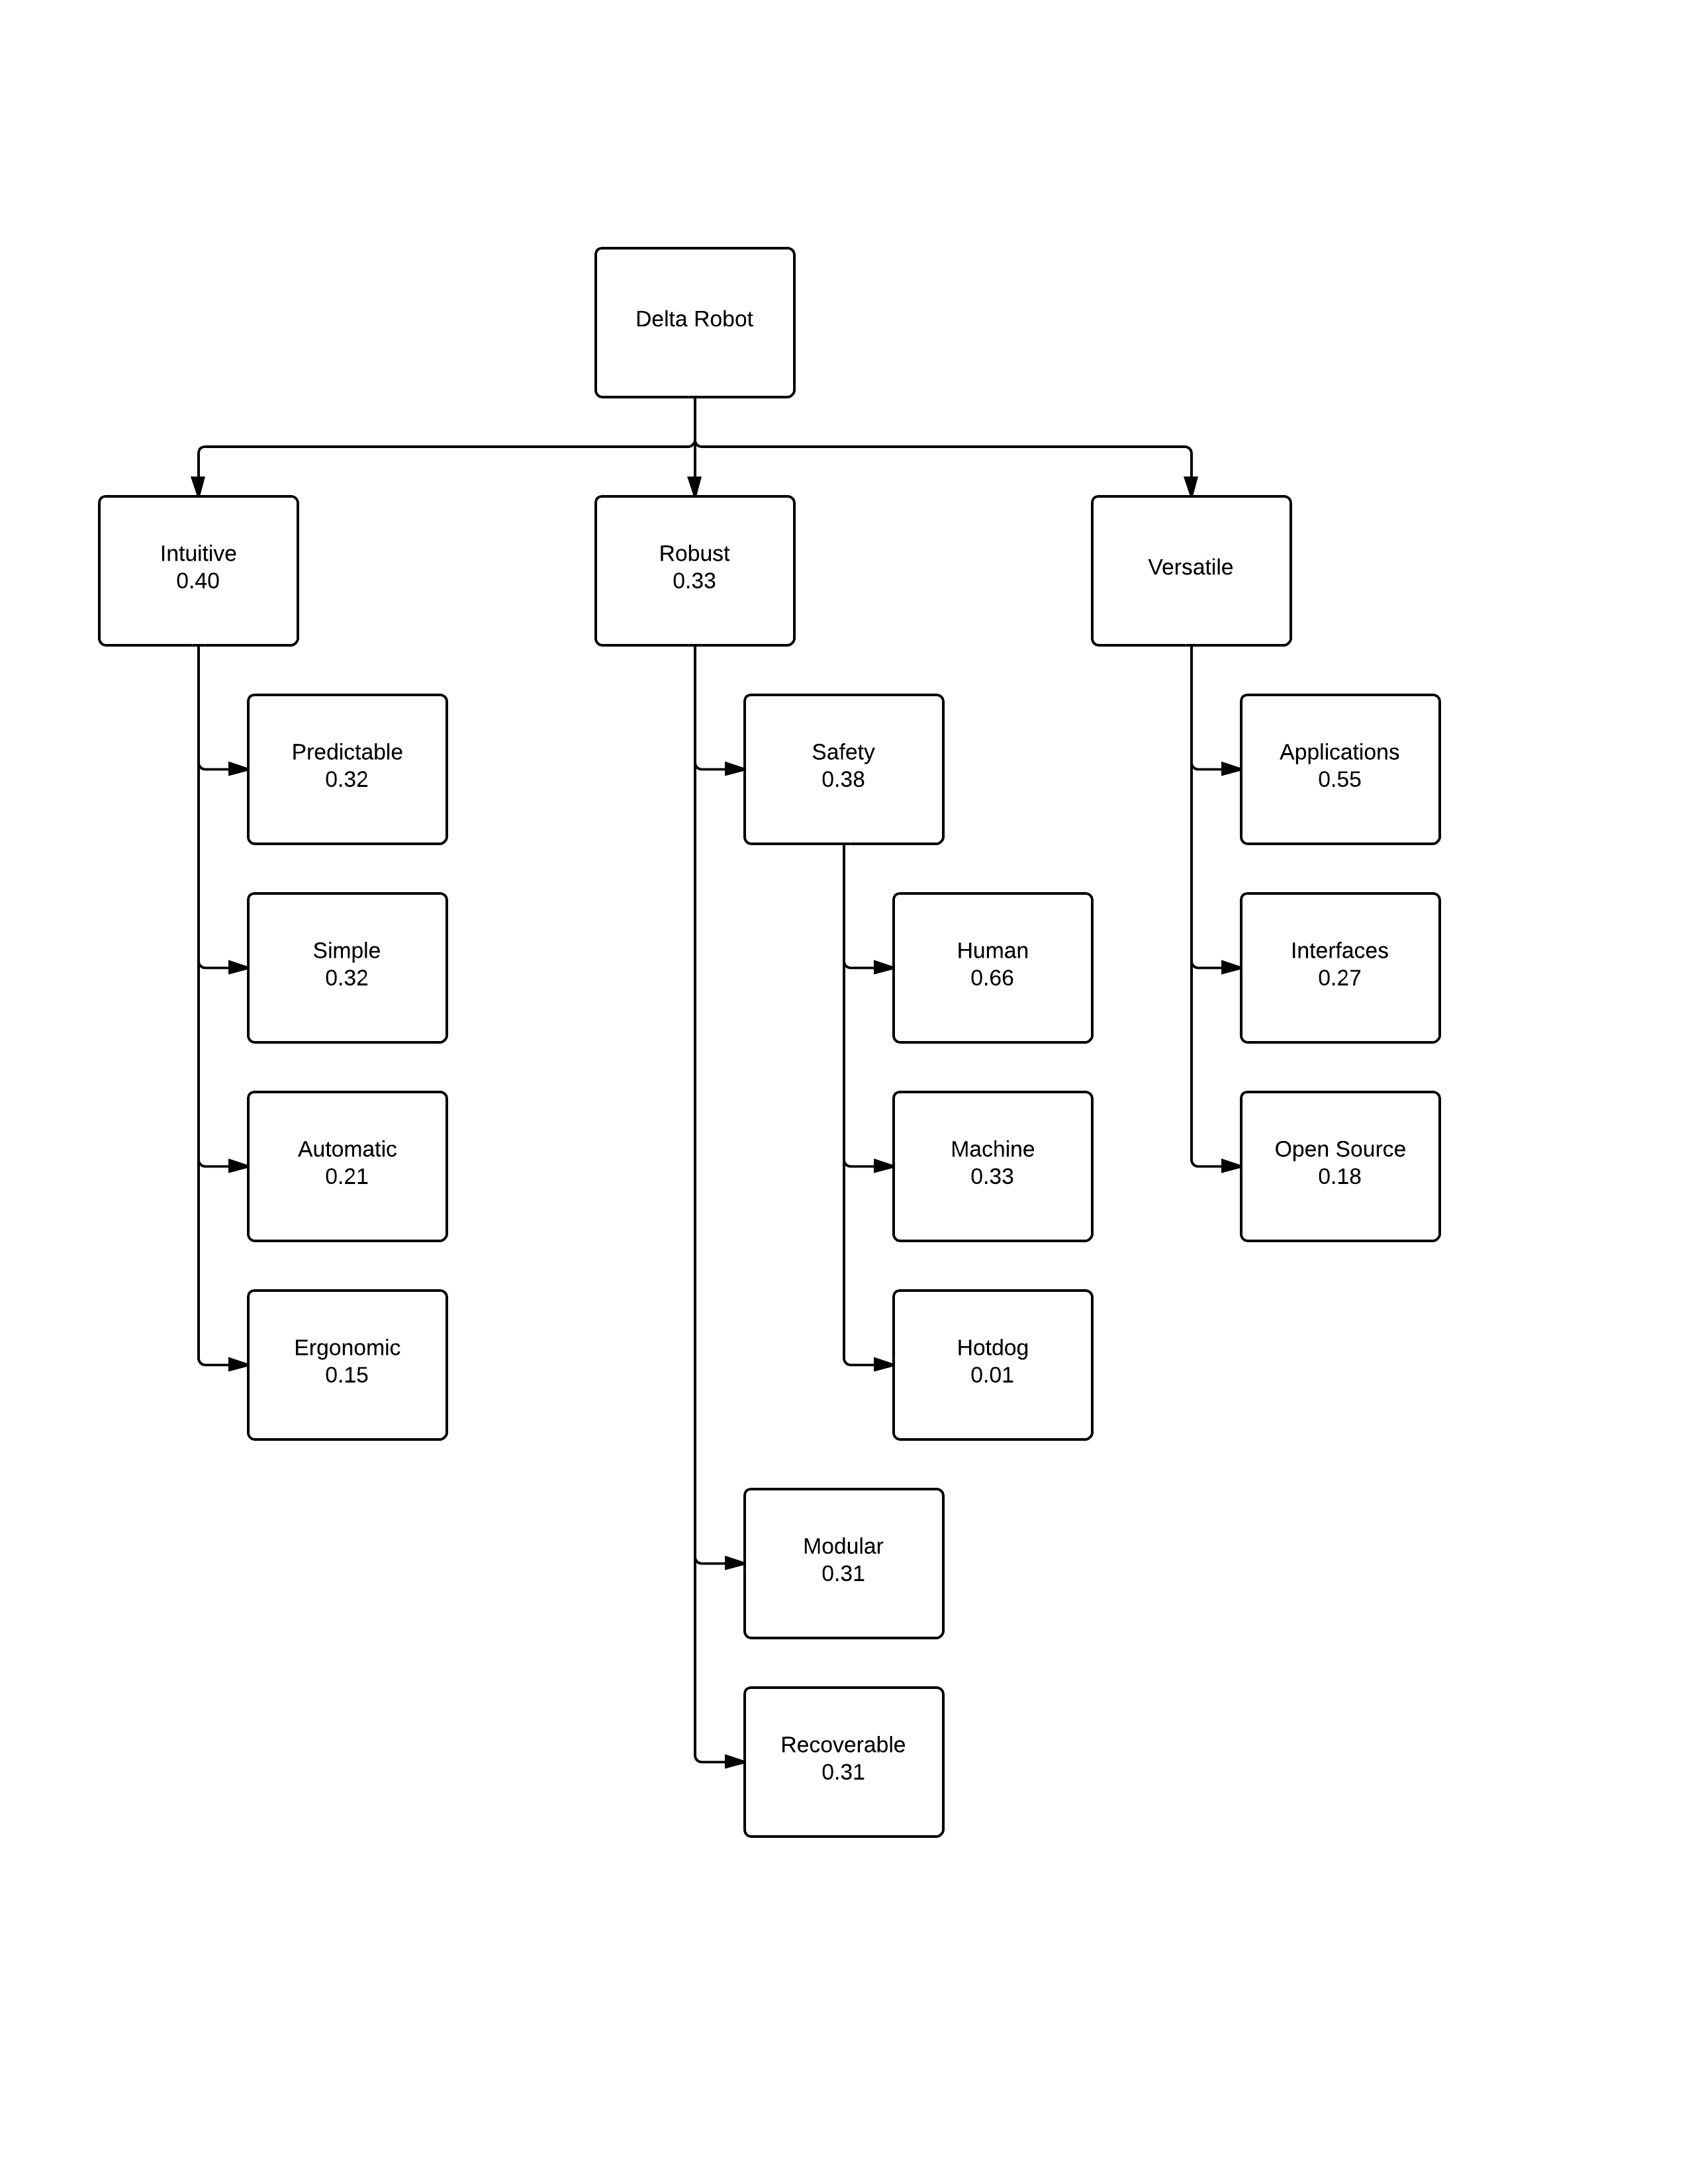
\includegraphics[width=0.8\textwidth]{objectivetree.png}
	\caption{Delta Robot Objective Tree}
	\label{fig:objectivetree}
\end{figure}

The three marketing requirement are Intuitive, Robust, and Versatile.
The most important marketing requirement is Intuitiveness, as the complexity involved with working in 3 dimensions makes it important for users to be able to operate in a manner that feels natural.
Components can be damaged if the robot is not operated in an expected manner.
It is also important for the robot to be robust.
This will help extend to robots work life and make failure less likely.
Finally, the robot must also be versatile.
While the focus of this project is \gls{pcb} repair, the delta robot platform will lend itself to many applications.
By creating this open source platform, others will be able to extend the usability of the delta robot.

\begin{table}[ht] 
	\caption{Primary Objective Definition}
	\label{table:primary}
	\centering 
	\begin{tabular}{c c c c c} 
		\hline\hline \\
		 			& Intuitive 	& Robust 		& Versatile 	& Total\\ 
		Intuitive 	& 1.00 		& 1.20 		& 1.50 		& 0.40 \\ 
		Robust 		& 0.83 		& 1.00 		& 1.25		& 0.33 \\ 
		Versatile 	& 0.67 		& 0.80 		& 1.00 		& 0.27 \\ 
	\end{tabular} 
\end{table}

\begin{table}[ht] 
	\caption{Intuitive Objective Definition}
	\label{table:intuitive}
	\centering 
	\begin{tabular}{c c c c c c} 
		\hline\hline \\
		 			& Predictable	& Ergonomic	& Simple 		& Automatic 	& Total\\ 
		Predictable 	& 1.00 		& 2.00 		& 1.00 		& 1.50 		& 0.32 \\ 
		Ergonomic		& 0.50 		& 1.00 		& 0.50		& 0.75 		& 0.15 \\ 
		Simple	 	& 1.00 		& 2.00 		& 1.00 		& 1.50 		& 0.32 \\ 
		Automatic	 	& 0.67		& 1.33 		& 0.67 		& 1.00 		& 0.21 \\ 
	\end{tabular} 
\end{table}

\begin{table}[ht] 
	\caption{Robust Objective Definition}
	\label{table:robust}
	\centering 
	\begin{tabular}{c c c c c} 
		\hline\hline \\
		 			& Modular 	& Safe 		& Recoverable	& Total\\ 
		Modular	 	& 1.00 		& 0.80		& 1.00 		& 0.31 \\ 
		Safe 		& 1.25		& 1.00 		& 1.25		& 0.38 \\ 
		Recoverable 	& 1.00 		& 0.80 		& 1.00 		& 0.31 \\ 
	\end{tabular} 
\end{table}

\begin{table}[ht] 
	\caption{Versatile Objective Definition}
	\label{table:versatile}
	\centering 
	\begin{tabular}{c c c c c} 
		\hline\hline \\
		 			& Applications& Interfaces	& Open Source	& Total\\ 
		Applications	& 1.00 		& 2.00		& 3.00 		& 0.55 \\ 
		Interfaces	& 0.50		& 1.00 		& 1.50		& 0.27 \\ 
		Open Source 	& 0.33 		& 0.67 		& 1.00 		& 0.18 \\ 
	\end{tabular} 
\end{table}

\section{Microprocessor Functionality}
The main microprocessor, an ARM Cortex 11 on the Raspberry Pi, will primarily be responsible for controlling the three stepper motors for the delta robot.
This objective will be achieved by creating a G-code interpreter written in C.
G-code is a standard way to instruct a \gls{cnc} router to move the work head throughout a \gls{3d} space, but is more complicated than accepting individual commands to move the motors.
The microprocessor will be responsible for scheduling movements to make smooth transitions to the destination, as interpreted from the G-code.

Instead of having physical buttons or a local user interface, the system will mainly be a network device, connected through WiFi or Ethernet.
The microprocessor will obtain G-code commands through local storage or by accepting G-code files over HTTP or SSH.
The G-code received over HTTP or SSH may then be optionally stored locally for faster use again in the future.
Execution of G-code sequences will be started through an HTTP interface, meaning any device with a browser can interact with the system.
All network interfaces will be password protected and use encryption algorithms to ensure that all commands executed are from authorized users. 

A secondary microprocessor may be required to control the tools on the delta robot, including the heat of a soldering iron, the rotation of a drill bit, or the positioning of cameras based on the user's position.
This secondary microprocessor will perform any required communication with the network-connected main microprocessor through a serial interface. 

\section{Telecommunications Functionality}
The telecommunications requirements for the project will involve sending data from the Oculus Rift to a centralized computed where it will be converted to movement data for the operation of the Delta Robot.
Video information must also be sent from the computer to the Oculus Rift.
The movement data will be transmitted from the central computer to the Delta Robot via Ethernet.
Video data from the Delta Robot will be transmitted to the computer by a video channel such a S-video.
The Oculus Rift will use a USB channel to transmit data to the computer while the computer will use a DVI channel to transmit the video data to the Oculus Rift.

\section{CEEN Appropriateness}
The senior capstone design project serves as part of the ABET accreditation for the CEEN program.
To meet these standards, students at the time of graduation will have:
\begin{enumerate} \parskip2pt
	\item The ability to apply knowledge of mathematics, science, and engineering. (ABET 3a)
	\item The ability to design and conduct experiments, as well as to analyze and interpret data. (ABET 3b)
	\item The ability to design a system, component, or process to meet desired needs within realistic constraints such as economic, environmental, social, political, ethical, health and safety, manufacturability, and sustainability. (ABET 3c)
	\item The ability to function on multidisciplinary teams. (ABET \gls{3d})
	\item The ability to identify, formulate, and solve engineering problems. (ABET 3e)
	\item The understanding of professional and ethical responsibility. (ABET 3f)
	\item The ability to communicate effectively. (ABET 3g)
the broad education necessary to understand the impact of engineering solutions in a global, economic, environmental, and societal context. (ABET 3h)
	\item The recognition of the need for, and an ability to engage in life-long learning. (ABET 3i)
	\item The knowledge of contemporary issues. (ABET 3j)
	\item The ability to use the techniques, skills, and modern engineering tools necessary for engineering practice. (ABET 3k)
\end{enumerate}

Through the design of the Delta Robot, all of these requirements will be met.
The design and construction will require the rigorous application of mathematics, science, and engineering for the software, hardware, mechanical, and system control. (ABET 3a).
Notably, the kinematics of the robot will require intense mathematical computations to ensure accuracy.
Experiments must be designed and conducted to ensure proper operation of components and the final result (ABET 3b).
The end result of the project will meet the needs outlined in the Background Summary (ABET 3c).
The level of success of the project will depend on how well the the team is able to cooperate and strive to achieve common goals (ABET \gls{3d}).
This project will present many engineering problems that will have to be solved (ABET 3e).
Not only must the group work towards common goals, but they must also communicate effectively (ABET 3g).
Similarly to ABET 3a, the entire project will involve the use of engineering skills that have been learned in previous coursework (ABET 3k).

The senior capstone project also serves as a culmination of the CEEN curriculum. Concepts and skills learned in previous courses must be applied in the design, construction, and documentation of the project.
Courses that will be built upon in the design of the Delta Robot are:
\begin{enumerate} \parskip2pt
	\item Microprocessor Applications
	\item Electrical \& Electronic Circuits
	\item Communication Systems
	\item Signals \& Linear Systems
	\item Digital Design \& Interface
	\item Microprocessor System Design
	\item Embedded Microcontroller Design
\end{enumerate}

In conclusion, the Delta Robot will prove a technically challenging project, requiring many of the skills taught throughout the CEEN curricula.
The completion of this project alone will meet at least 7 of the 11 ABET accreditation criteria.

\section{Constraints}	
Constraints for this project are as follows:

\subsection{Identification}
Most notable among the constraints to be outlined for this project are time and money.
As full-time students with part-time jobs, time is to be split among many areas in the next 7-8 months.
Therefore, hours must be carefully scheduled as a group for work on the project.
Much of the time spent working will have to be on an individual basis.
The scope of the project must be carefully decided so as to not accrue an impossible time requirement. 
This 2014 Capstone Project is funded entirely by the engineering team. 
Again, as full-time students with part-time jobs, funds are limited.
Therefore, cost will play a significant role in determining which components to buy.
Solutions must be carefully planned in order to avoid rework and wasting money spent.

Other constraints will be safety, manufacturability, robustness, and versatility as described in the Background Summary.

The primary resources for the project are the four engineers involved with the undertaking.
The engineers will be responsible for all design and implementation.
Other resources that will be used include a senior thesis office that will be the primary work space, and a \gls{cnc} \gls{pcb} mill that will be used for prototyping.

\subsection{IEEE Standards}
The following IEEE standards will be adhered to when appropriate:
\begin{enumerate} \parskip2pt
	\item IEEE Std 830-1998/IEEE Recommended Practice for Software Requirements Specifications
	\item IEEE Std 1220-2005/Standard for Application and Management of the Systems Engineering Process
	\item IEEE Std 1490-2011/A Guide to the Project Management Body of Knowledge
\end{enumerate}

\subsection{Preliminary Budget}
A preliminary budget of \$2500 has been appropriated, but is subject to change.
The breakdown is shown in Table ~\ref{table:budget}.
The bulk of the cost of the project will be mechanical parts such as belts, rods, fasteners, etc.
The next greatest expense is expected to be electronic components.
Most software required is expected to be freely available, but funds have been left under 'unallocated' should this be nessescary.
Finally 'Systems' has received a budget of \$500 for acquiring the assembled technology necessary to implement the project. 

\begin{table}[ht] 
	\centering 
	\begin{tabular}{c c c} 
		Designation	& Funds 		& Percentage\\
		\hline
		Mechanical	& \$1,000 	& 40.0\% \\ 
		Electrical	& \$500 		& 20.0\% \\ 
		Systems		& \$500 		& 20.0\% \\ 
		Unallocated	& \$500 		& 20.0\% \\
	\end{tabular} 
	\caption{Preliminary Design Budget}
	\label{table:budget}
\end{table}

\subsection{Engineering Hours}
In comparison to the scope and time required of previous capstone design projects, an estimated 1000 work hours will be needed to complete this project.
This number corresponds to approximately 8 hours per week per person involved with this 2014 Capstone Project.

\chapter{Project Charter}
\section{Project Approach}
The purpose of this project is to create a final working system that not only meets, but exceeds, the expectations of all stakeholders. This goal will be achieved through proper planning and execution by talented engineers with a focus on system testing throughout the process.

\subsection{Roles and Authority}
The following definitions will serve as the guidelines for each team member's major tasks throughout the project lifetime. All team members are expected to help one another out to ensure the best outcomes for the project, not just for the individual's task completion
\paragraph{Faculty Sponsor: Herbert Detloff}
Demonstrates previous experience with several successful capstone design projects.
Provides feedback and assessment of project definition, plan, and status.
Ensures that all team members are aware of the engineering impact of the project on the University of Nebraska - Lincoln and the rest of the world.
Teaches standard engineering principals for project management, development, execution, and testing to aid in the project's completion.

\paragraph{Resource Manager: James Gehringer}
Responsible for promoting collaboration, communicating progress with the faculty sponsor, and procuring resources.
Accountable for intellectual property management in solidification of ideas and iterative verification of project objectives.
Involved with all phases of design in order to better assure both long and short term goals are met with efficiency by keeping track of the progress of the project by setting deadlines, scheduling tasks, and monitoring progress through tools such as Gantt charts.
Oversees documentation and monitors project health to identify issues as soon as possible.

Reports to the Faculty Sponsor. 

\paragraph{Systems Engineer: Evan Milton}
In charge of generating the system's requirements and specifications and understanding the project as a whole, including mechanical, electronic, and software components and their interfacing.
Works closely with the Hardware and Software Development Engineers to best meet the team objectives, system's requirements, and specifications.
Responsible for acceptance testing the prototypes and final project to ensure quality and confirm that all specifications are met.
Determines alternate solutions case any solution fails or becomes unfeasible during development.
Makes final design decisions when challenges arise that require major modifications.

Reports to the Resource Manager and Faculty Sponsor.

\paragraph{Hardware Development Engineer: Chad Staley}
Accountable for developing the design, layout, construction, and testing of the electrical systems required for this project to create a solid platform for the software.
Focused on simplicity and robustness in design, to aid troubleshooting when software is added to the project.
Understands and can communicate the software interfacing that must occur to make the hardware function properly.

Reports to the Systems Engineer, Resource Manager, and Faculty Sponsor. 

\paragraph{Software Development Engineer: Josh Dewitt}
Responsible for the higher level functionality of the project by writing clean, modular code that can be adapted where hardware changes might be cost-prohibitive.
Will communicate with the Hardware Development Engineer to understand the hardware interfacing to meet the requirements set by the Systems Engineer.
Performs domain, software element, and requirements analysis to ensure the code produced matches the needs of the users, then develops code in any language necessary, using test­-driven development.

Reports to the Systems Engineer, Resource Manager, and Faculty Sponsor.

\subsection{Quality Objectives}
The team agrees that output of this capstone design sequence will be high-quality product that is reproducible, robust, and goes beyond expectations.
This objective will be achieved by setting engineering requirements that will use all of our talent, while still being achievable given the time frame of the course, and meeting these set requirements through a team effort.
Rapid prototyping will allow issues to be revealed early in the project's execution, making sure that the correct priorities are set to focus on those items that may cause an engineering requirement to not be met.

\section{Risk Management}
Certain risks will be faced throughout the project, though proper avoidance and mitigation plans will allow project objectives to be completed on time.
Risks will be obsessed using AHP and pairwise comparisons.
If possible, quantitative measurements, in terms of financial or class grade loss if the risk is realized, will allow comparison to determine which risks should be focused on to ensure that they are not realized.

\subsection{Risk Identification}
From previous experience, the major risks that will occur in the project will likely be related to increasing scope, unfeasible designs, insufficient resources, delayed shipments, and lack of motivation.

\subsection{Risk Avoidance}
\begin{itemize} \parskip2pt
	\item To avoid increasing scope late in the project, there will be a change moratorium to the project’s scope at the end of the senior thesis proposal class. Any additional substantial features must be put on hold until the end of the semester if time permits; all other requirements must first be completed.
	\item To avoid issues from a design becoming unfeasible, viable alternative designs will be created in the planning phase.
	\item To avoid running short of resources, proper resource management and thorough time and money planning will ensure that all resource expenditure is within budget.
	\item To avoid being affected by delayed shipments, parts will be ordered as soon as they are confirmed to be required.
	\item To avoid slipping motivation, the team will be kept in contact to create an atmosphere of team cooperation and ensure that all team members feel useful in the project.
\end{itemize}	

\subsection{Risk Mitigation}
\begin{itemize}
	\item In the case of required increased project scope, the team will collaborate and decide the new priority of tasks using AHP. The tasks will be worked in the order decided, and the team will understand which items may not be completed in time.
	\item In case a design becomes unfeasible, one of the alternate designs created in the planning phase will be pursued.
	\item In case of insufficient financial resources, the investors will be contacted, or more investors will be located to sponsor the project.
	\item If shipments are delayed, alternative distributors will be researched and ordered from to obtain the part in time.
	\item If there is a lack of motivation on the team, team outings will be planned that do not involve the project, but will allow team bonding and any personal issues to be discussed.
\end{itemize}

\section{Project Control}
The project will focus on the punctual production of functional deliverables at set deadlines, tracked in a Gantt chart.
The Resource Manager will be able to concretely monitor project status, and inform members of changes in course as they become necessary.
Detailed documentation of all efforts will be maintained in each person's engineering logbook.

\subsection{Communication Channel}
Face-to-face group status meetings in PKI 330G will be held to update the status of each deliverable being worked on and provide proactive feedback to keep the project on track.
As much communication as possible should be done in person, as opposed to through phone, text, or email conversations because of the higher information bandwidth.
To aid in keeping track of status of individual kanbanpad.com, an online project tracking tool will be used to update the status of tasks between the planning, designing, development, testing, and release phases of project development.
Room PKI 330G will be used for any additional meetings required, which may or may not include the entire team.

\subsection{Communication Frequency}
The face-to-face status meetings will be held twice a week to keep each member aware of the overall progress.
All team members are encouraged to use PKI 330G as the primary work area for the project to increase collaboration and encourage spontaneous discussion regarding the project.
All team members should update the status of their tasks on kanbanpad.com as soon as they change between one of the stages, allowing all members to see the most up-do-date project status wherever they are.
\end{document}
